\chapter{Experiment}
\label{ch:experiment}

In the Experiment an optical transmitter was simulated in OptSim. The Experiment was divided in three sub-projects.

\section{Project 1}
\label{sec:P1}

\begin{figure}[h]%
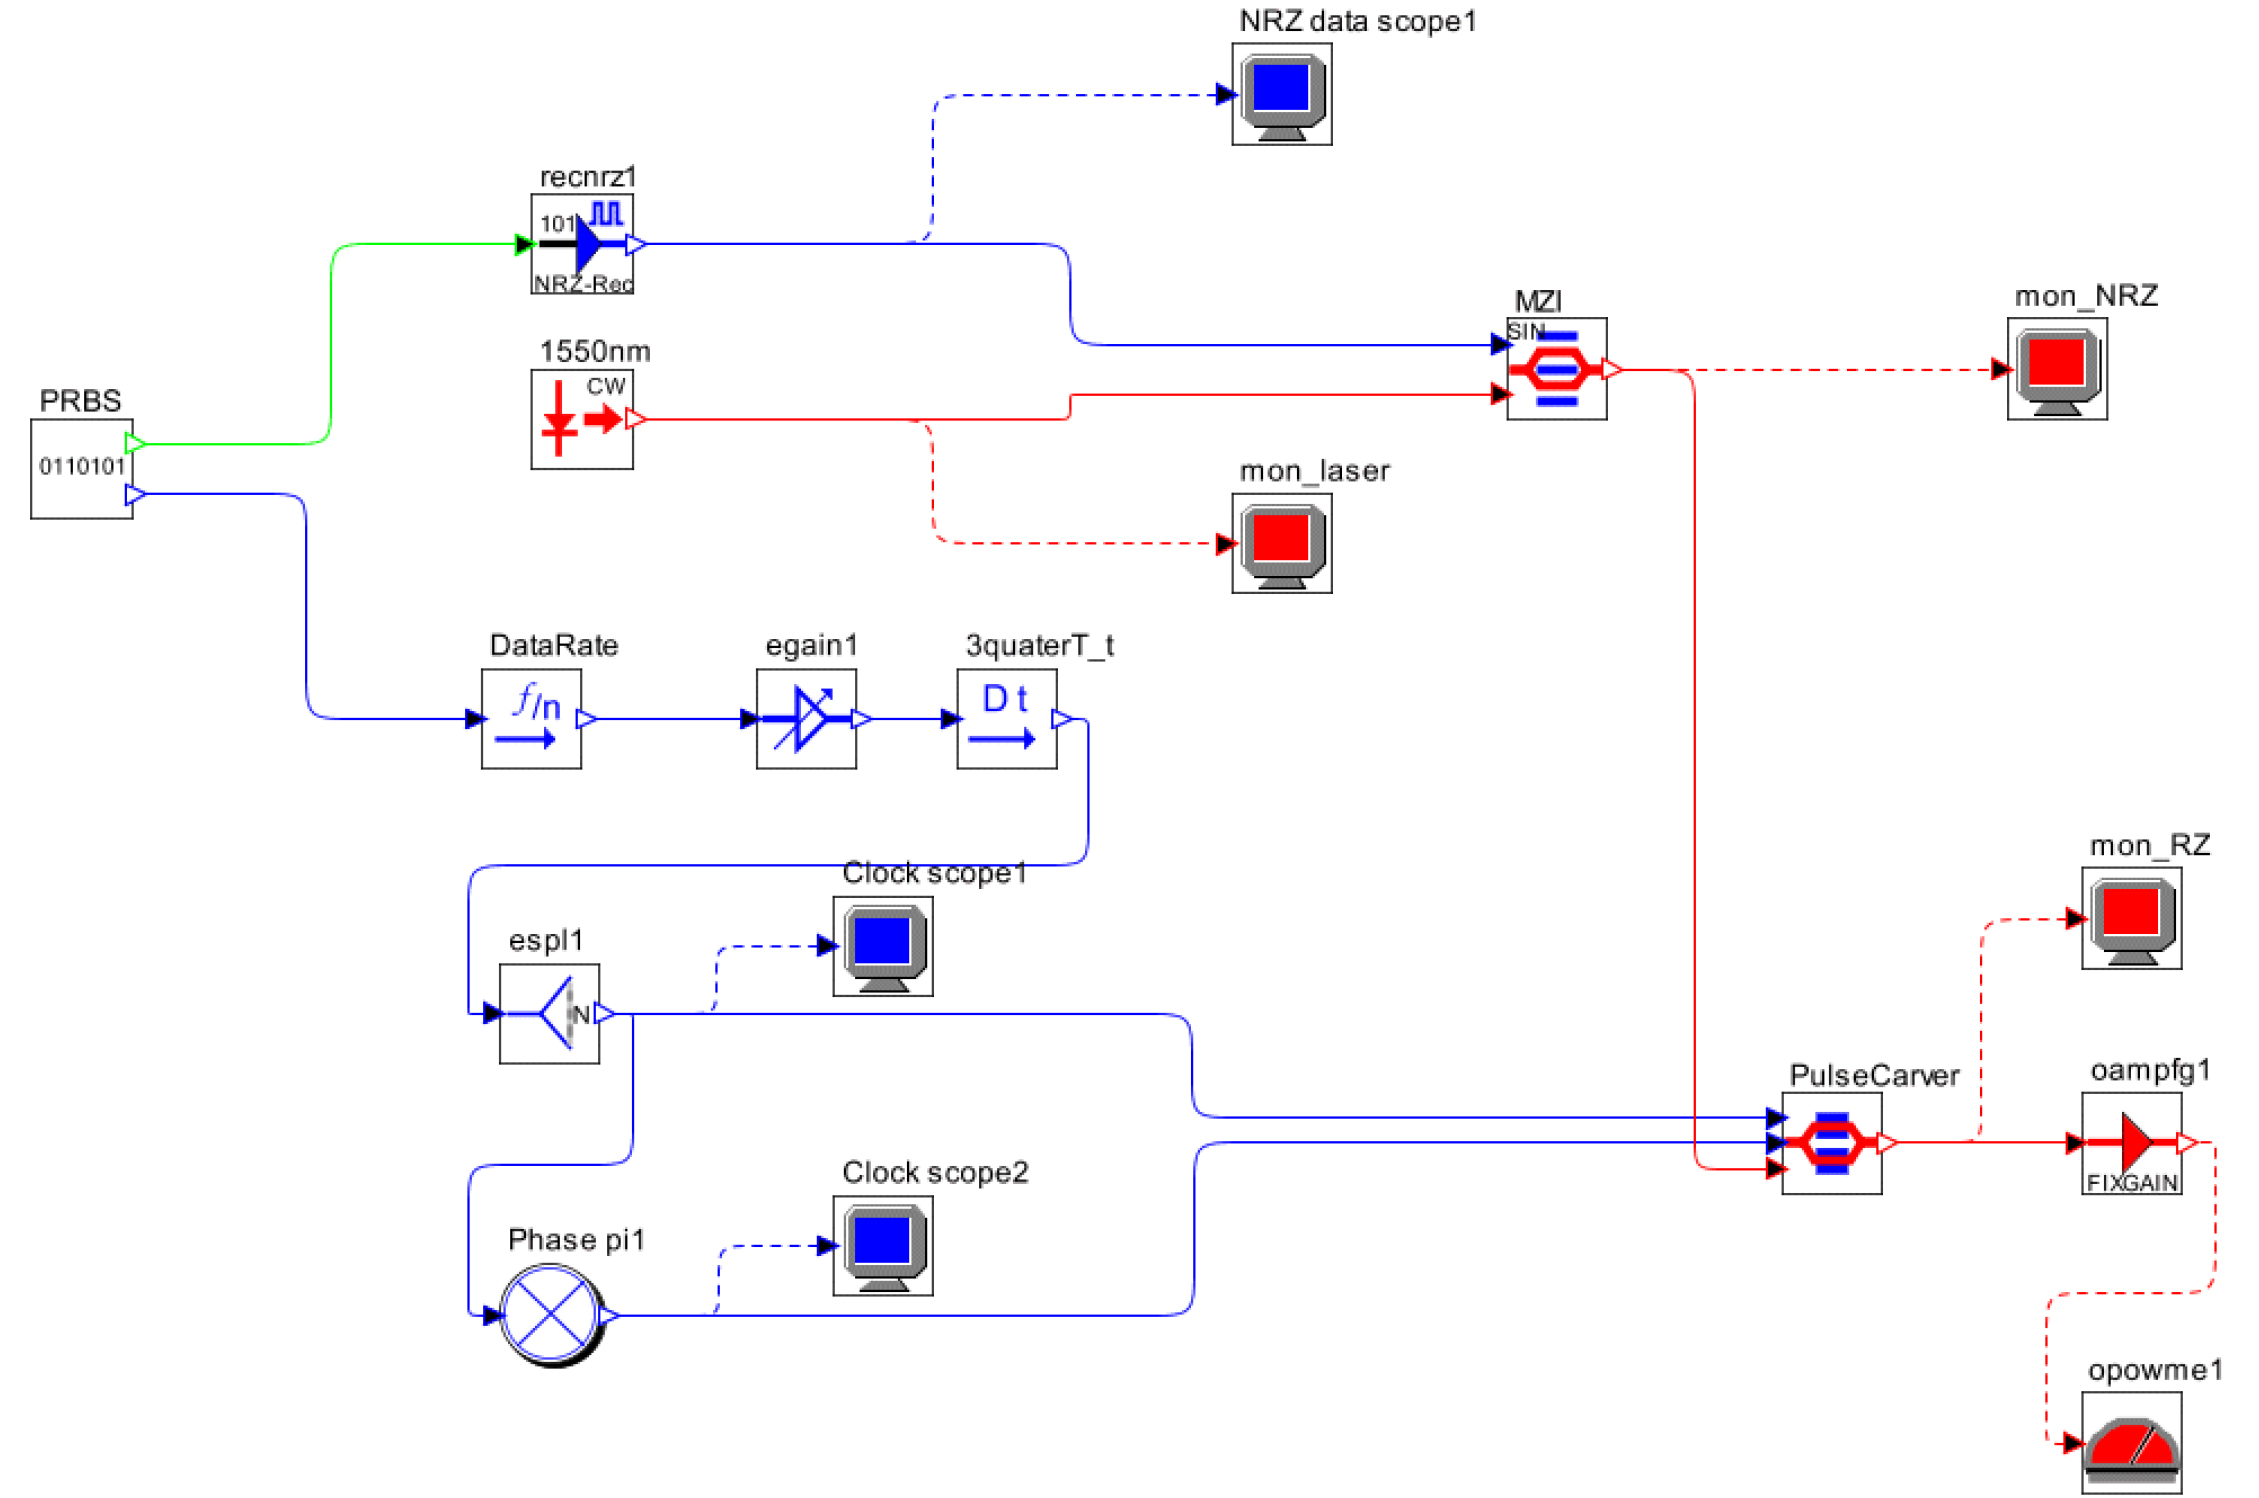
\includegraphics[width=.8\columnwidth]{Grafiken/P1_aufbau.jpg}%
\caption{Schematic: OptiSim Sample-Mode example of a 50~\% RZ-OOK-Transmitter}%
\label{fig:P1_aufbau}%
\end{figure}

For the Experiment an OptiSim Example of a 50~\% RZ-OOK-Transmitter was used. Figure \ref{fig:P1_aufbau} shows the schematic of this example\footnotemark[3]. In the upper left-hand side there's the PRBS which generates a pseudo-random bit-stream. A logical connection path (green) leads to an NRZ-Rectifier (recnrz1) which generates an electrical output signal. Via an MZI this electrical NRZ-signal gets modulated on a 1550~nm laser. 

Starting in the upper left-hand side at the PRBS again, the lower path leads to an divider. Here the DataRate can be divided. In the first project there is no change of the data rate and the divider is 1. Afer that there is an amplifier (egain1) and a time-delay element. Those elements are used to set the driving-voltage for the MZM (PulseCarver).

For driving the MZ in "`push-pull"' mode (cf. \ref{sec:MZM}) the phase of one electrical paths is shifted. The folloing MZM (PulseCarver) is used to carve the NRZ pulses to a NRZ-OOK signal. \footnote[3]{Materials for the Preparation of Experiment 7: Simulation of Optical Transmitters}

Figure \ref{fig:P1ExB_Spectra} shows the spectrum of the laser source (red) and the spectrum of the optical NRZ signal (green). At a frequency of $f~\approx~193.415$~THz both spectra show a large peak. This is the laser frequency and therefor also the carrier frequency of the NRZ-Signal. 10~GHz beside the carrier frequency are the peaks of the 10~Gbit/s NRZ signal and it's harmonics. 

\begin{figure}%
\centering
%\begin{adjustwidth}{0cm}{0cm}
	\subfloat[Spectra]{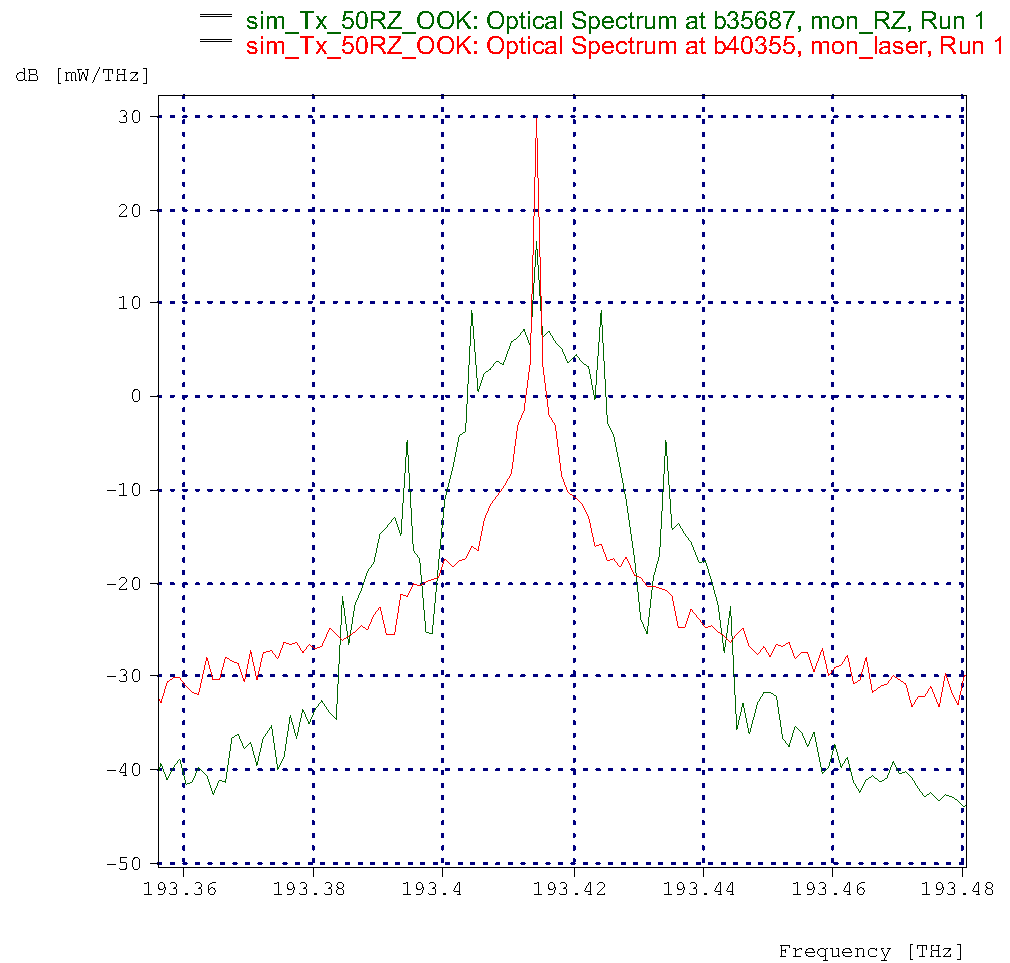
\includegraphics[totalheight=6 cm]{Grafiken/P1ExB_Spectra.pdf}\label{fig:P1ExB_Spectra}~}
	\subfloat[Eye Diagramm]{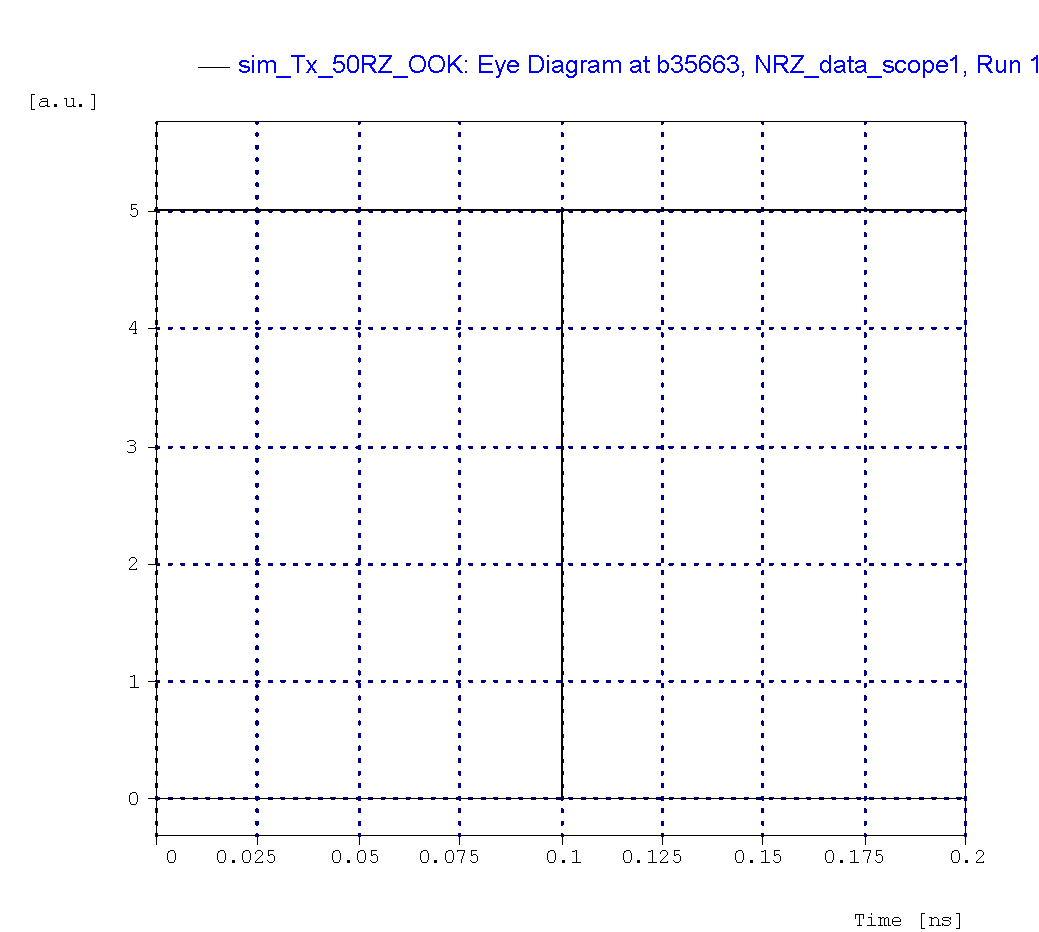
\includegraphics[totalheight=6 cm]{Grafiken/P1ExB_Eye.pdf} \label{fig:P1ExB_Eye}}%
%\end{adjustwidth}
\caption{\textbf{a)} Spectrum of the laser source (red) and spectrum of the NRZ-signal (green). \textbf{b)} Eye diagramm of the NRZ signal.}%
\label{fig:P1ExB_1}%
\end{figure}

Figure \ref{fig:P1ExB_Eye} shows an eye diagramm of the generated NRZ signal. Since a digital signal is regarded, the slopes of the signal are perfectly steep.
\comseb{evtl noch irgendwas}
Figure \ref{fig:P1ExB_bit} shows the electrical , the optical NRZ  and the optical 50~\% RZ bit sequenze. Both optical sequences match the electrical signal. The RZ signal shows an errorous pulsshape, because the exported data of this signal has not enough datapoints. Figure \ref{fig:P1ExB_FWHM} shows the correct shape of one pulse. In this figure also the full width at half maximum can be measured. With an FWHM of 0.05~ns and a lenght of a bitslot of 0.1~ns the duty cycle of the optical signal is 50~\%.

\begin{figure}%
\centering
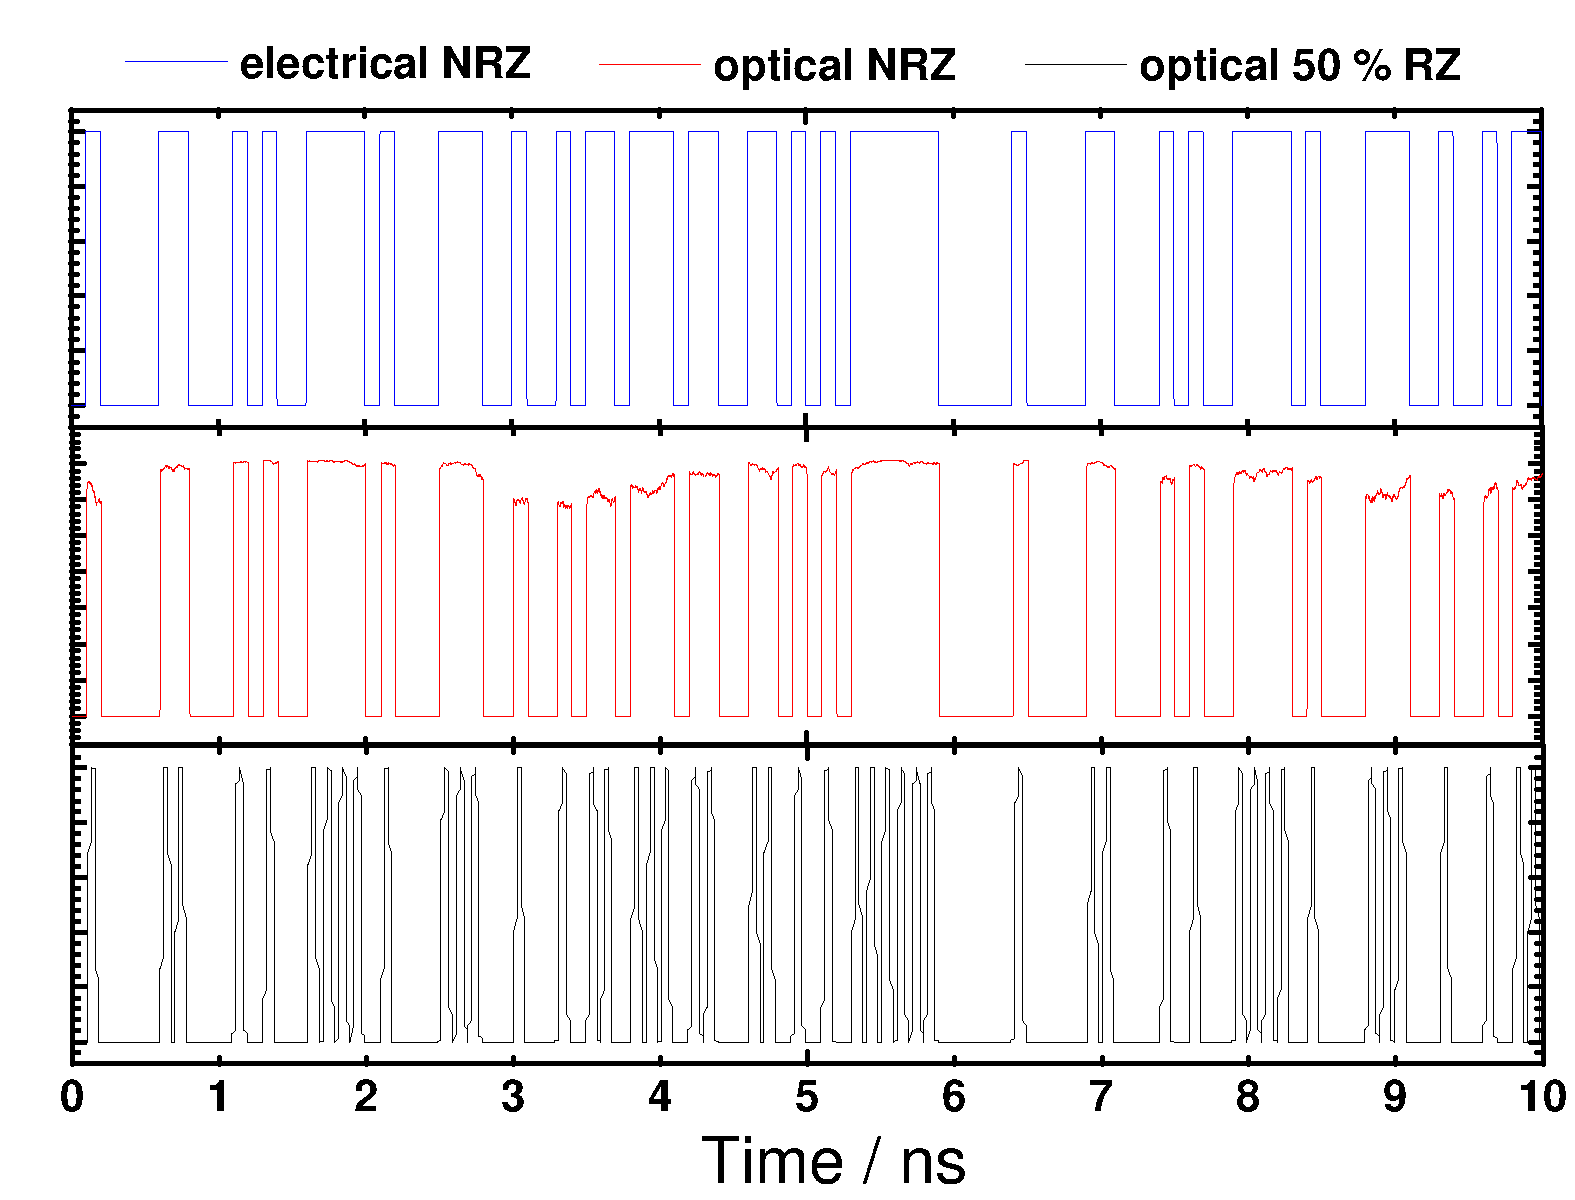
\includegraphics[width=.8\columnwidth]{Grafiken/P1ExB_BitSequence.pdf}%
\caption{NRZ bit sequences.}%
\label{fig:P1ExB_bit}%
\end{figure}

\begin{figure}%
\centering
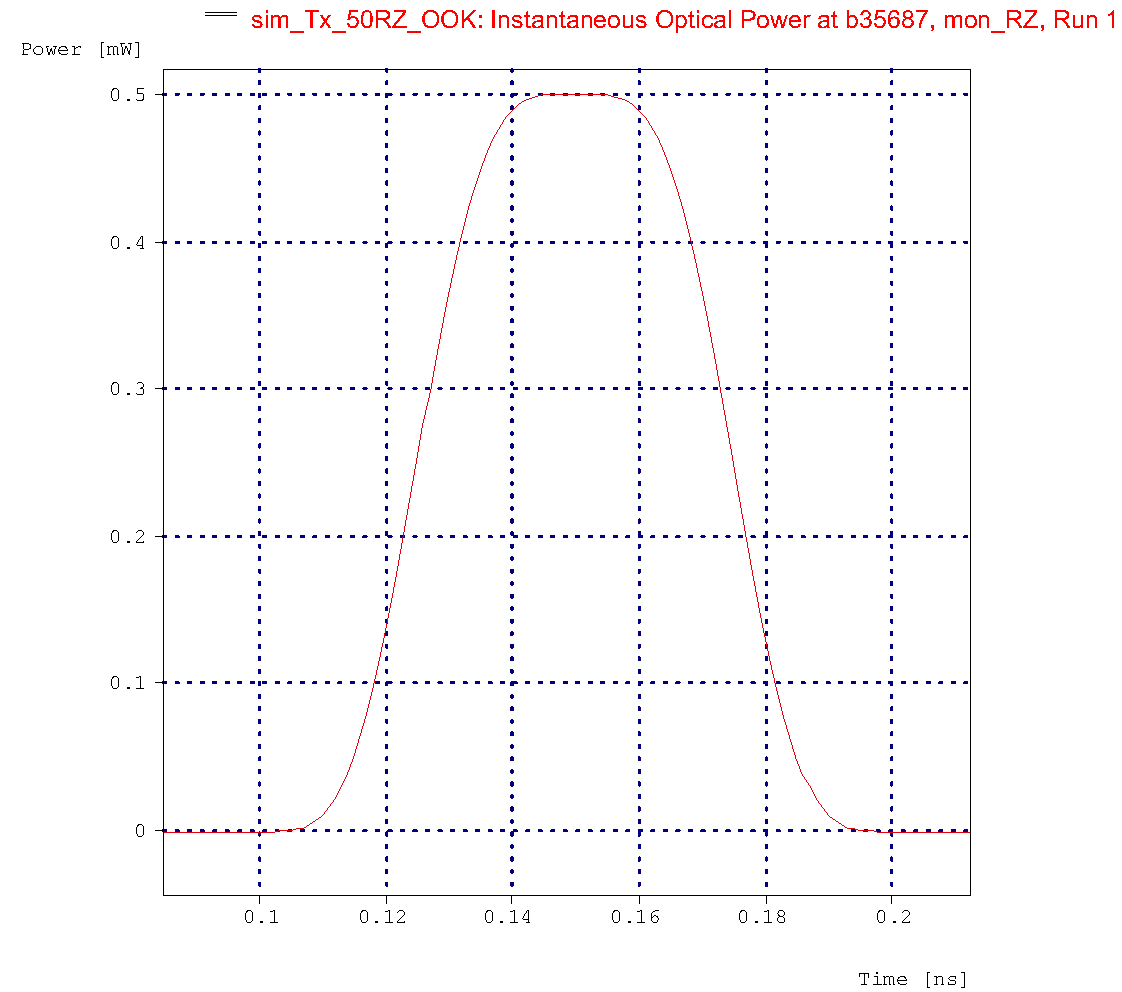
\includegraphics[width=.5\columnwidth]{Grafiken/P1ExB_FWHM.pdf}%
\caption{50~\% RZ OOK Pulse}%
\label{fig:P1ExB_FWHM}%
\end{figure}

To design an optical transmitter outoput of 33~\% RZ OOK pulses the parameters of the optical tranmsmitter were changed. 
The operation of the pulse carver was change to carve the NRZ signal to a 33~\% RZ OOK signal. The driving voltage of the MZM needet to be changed. Therefore the Offset Voltage was set to 0~V. As in \ref{sec:RZ} the driving voltage needs to be doublet comparted to the 50~\% signal.To do this the gain (lin) (egain1) was set from 2.5 to 5.0. The driving frequency needed to be halved by setting the N-division factor (DataRate) to 2.
At least the phase of the driving signal was adapted by setting the time delay (3quarterT\_t) to 0,75/0,01 (ps).

The now generated signal shows pulses with a FWHM of 0.03~ns.



\section{Project 2}
In the next Project two PIN photodetectors with default parameters were inserted. One at the exit of the NRZ-MZM and the other after the optical amplifier("`oampfg1"') for the RZ signal. To display the signal a "`Electrical Monitor"' was placed behind each of the detectors. After running the simulation the eye diagrams of each signal were recorded. In the eye diagram of the NRZ signal the influence of the photodiode can be seen. The transition from "0" to "1" and vice versa is not instant anymore (cf.\ref{sec:P1}). Since the RZ-signal is rising and falling in one bitslot anyway, it is influenced less by this effect. 

For the Q-factor a value of 40~dB is obtained. \todo{is this value practical}

\begin{figure}%
\centering
%\begin{adjustwidth}{0cm}{0cm}
	\subfloat[Eye Diagram NRZ]{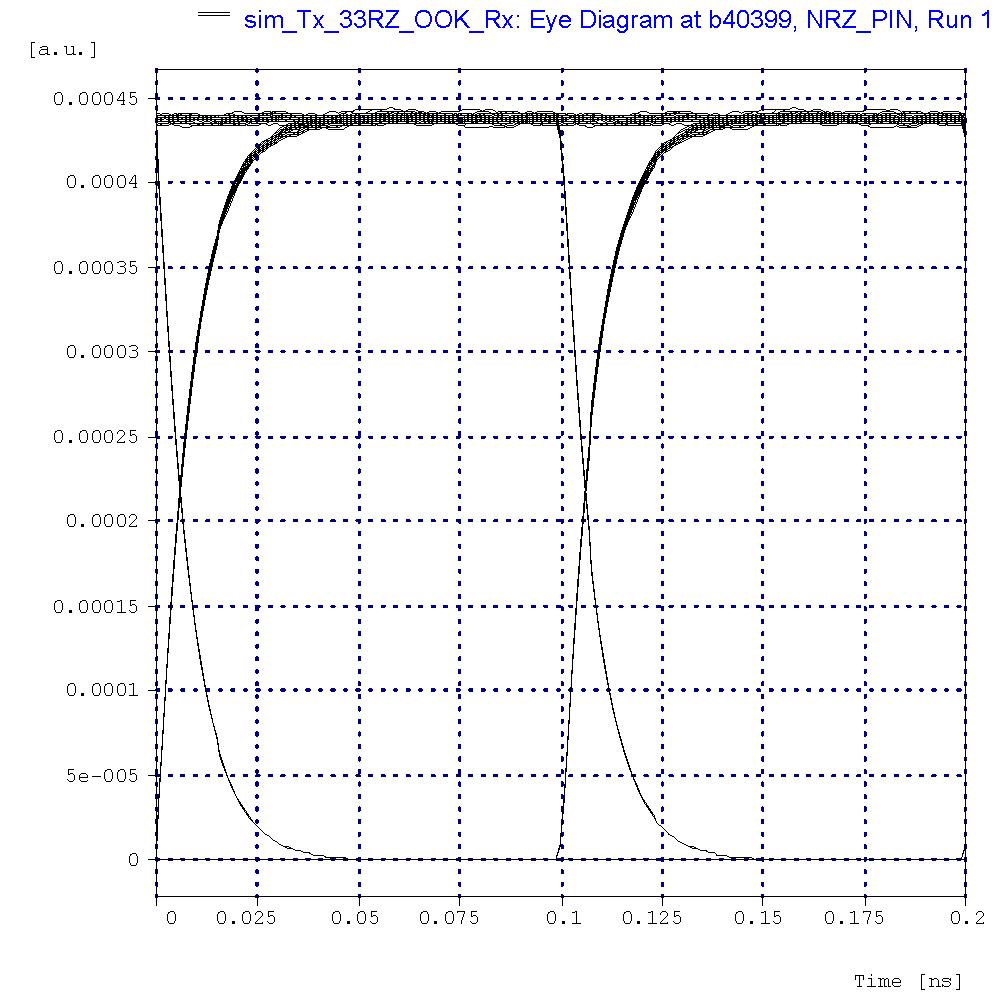
\includegraphics[totalheight=6 cm]{Grafiken/P2_ExA_NRZ_PIN_eye.pdf}\label{fig:P2ExA_Eye}}
	\subfloat[Eye Diagram 33\%-RZ]{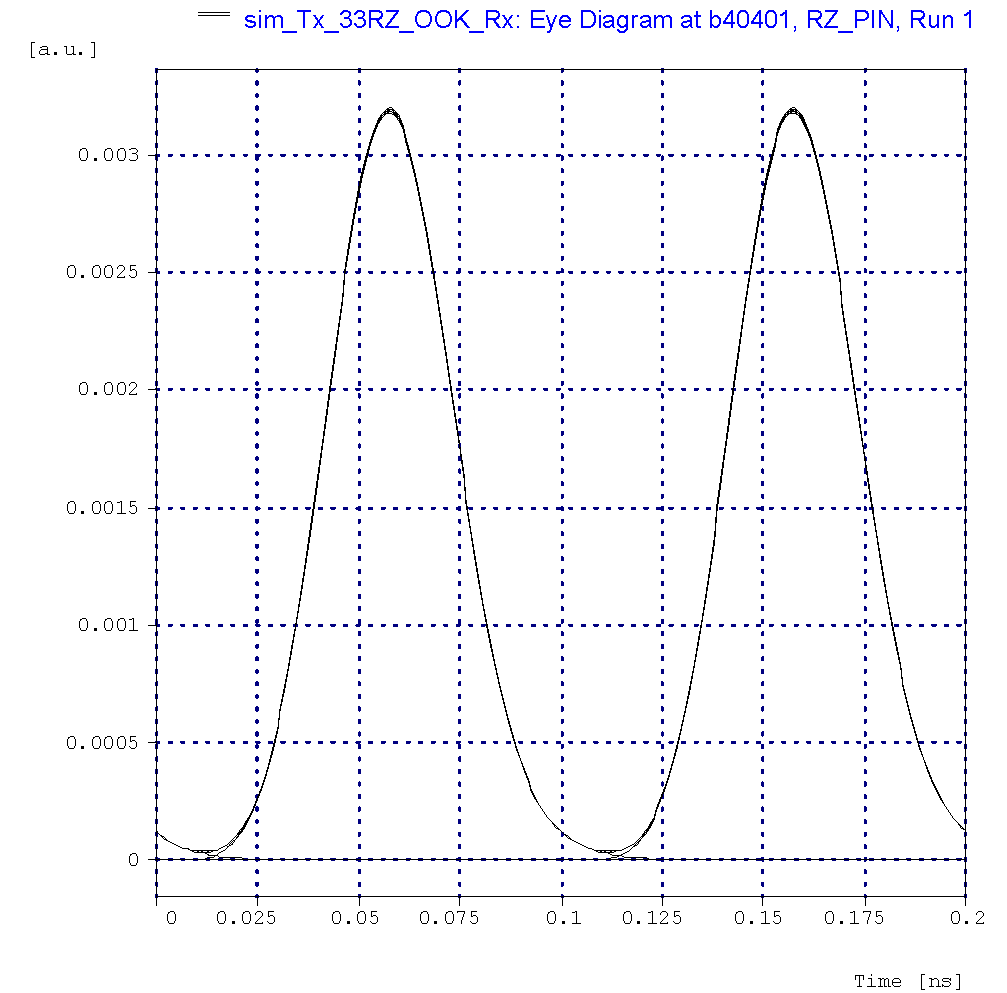
\includegraphics[totalheight=6 cm]{Grafiken/P2_ExA_RZ_PIN_eye.pdf} \label{fig:P1ExA_Eye}}%
%\end{adjustwidth}
\caption{}%
\label{fig:P2ExA_1}%
\end{figure}

OptiSim gives several possibilities to change parameters of the PIN-diode. 
By changing the quantum efficiency of the diode the output amplitude varies. A large quantum efficiency leads to a higher, a small quantum efficiency leads to a lower output amplitude. 

Changing the -3~dB bandwidth changes the reaction time of the diode. 
Figure \ref{fig:P2ExB_3dB} shows the output signal of the PIN-diode for different -3~dB bandwidths. To demonstrate this effect an incoming optical NRZ signal was used. A bandwidth of 10~GHz (cf. fig. \ref{fig:P2ExB_10}) leads to a rise-time of approximately 0.03~ns. \comwo{ich hab jetzt mal von einer hilfslinie �ber null bis eine hilfslinie unter max gemessen :-/.. grob}

A -3~dB bandwidth of 40~GHz (cf. fig. \ref{fig:P2ExB_40}) leads to much faster rise and fall times. Here the rise time is about 0.01~ns. The same behaviour can be observed for the fall time.
\todo{Muss hier rein warum das so ist??}

\begin{figure}%
\centering
%\begin{adjustwidth}{0cm}{0cm}
	\subfloat[10~GHz]{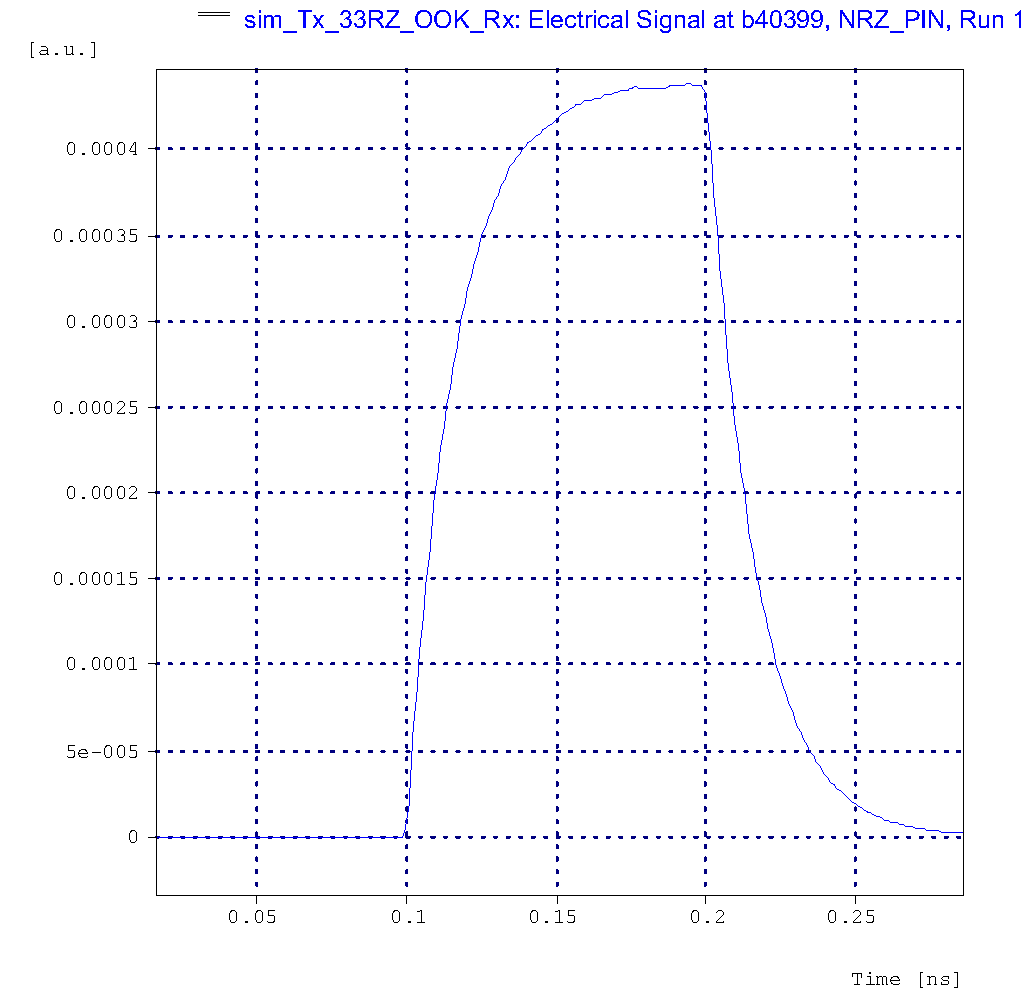
\includegraphics[totalheight=6 cm]{Grafiken/P2ExB_10.pdf}\label{fig:P2ExB_10}~}
	\subfloat[40~GHz]{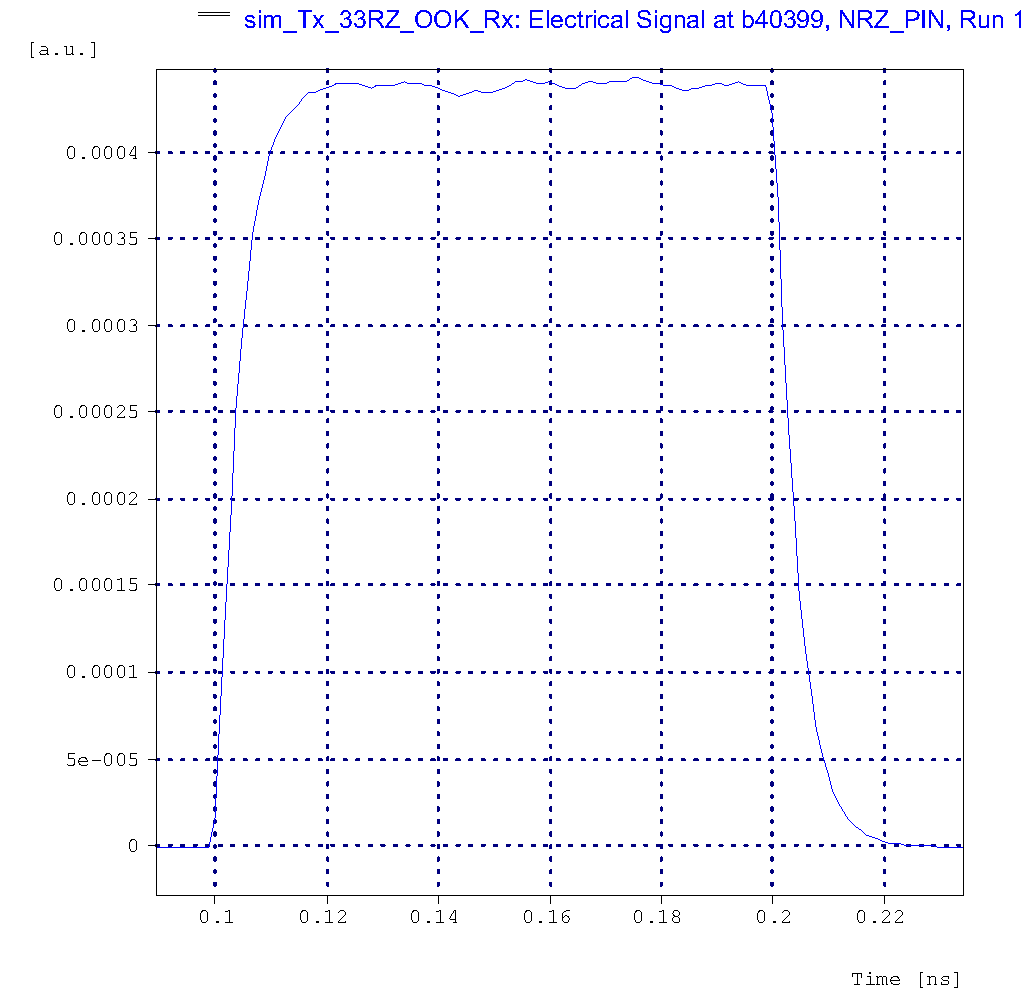
\includegraphics[totalheight=6 cm]{Grafiken/P2ExB_40.pdf} \label{fig:P2ExB_40}}%
%\end{adjustwidth}
\caption{The rise- and fall time of the signal depends on the -3 dB bandwidth (\textbf{a)} 10~GHz and \textbf{b)} 40~GHz) of the PIN-diode.}
\label{fig:P2ExB_3dB}%
\end{figure}




\section{Project 3}
\label{sec:P3}
In Project 3 an additional fibre was added to the simulation. The fibre "`CorningSMF28\_1550"' was inserted between the Pulse Carver and the in project 2 added PIN diode. 
\todo{What parameters do we know?}\comwo{Muss das wirkilich rein?}

For this project all nonlinear effects were deactivated ("`Advanced control"' -> all options were switched off).

To achieve an optical power of 0~dBm out of the fibre the optical power of the sender laser needed to be adjusted. Without adjusting the power, there is a power of -3.304 dBm after the 10~km fibre. Setting the CW-Power of the 1550~nm Laser to 3.304 dBm leads to an optical output power of 0 dBm after the 10~km optical fibre.

Figure \ref{fig:P3ExB_Eye10} shows the eye diagram after 10~km of transmission line. Figure \ref{fig:P3ExB_Eye20} shows he eye diagram after 20~km transmission line. Through the dispersion, there is an overlap of two neighbouring "`1s"'. At a fiber length of 10 km this overlap is marginally low. At the length of 20~km the overlap increases significantly. Hence this overlap only occurs for two neighbouring "1s" it will not lead to problems in the signal detection. If the broadening of the pulse is increased, the overlap even occurs in the bitpattern "101". Then it is possible, that the "0" between the "1s" is interpreted as a "1". 
\comseb{Ich bin mir net sicher ob das stimmt. das hab ich mir so �berlegt}

Figure \ref{fig:P3ExB_Q} shows the \textit{Q}-factor of different fibre length. After 10~km the \textit{Q}-factor is 39.99~dB. With increasing fibre length the \textit{Q}-factor decreases. Figure \ref{fig:P3ExB_Q} shows in the measured range a linear dependency between \textit{Q} and the fibre length. At 20~km \textit{Q}~=~34.40~dB, at 30~km $Q=29.66$~dB and at 40~km $Q=24.27$~dB.
\todo{how are the q-factors measured}
\comwo{argh... das ist auch arg aus dem finger gesaugt, schau lieber nochmal dr�ber als standardabweichungsexperte... vergleiche 22.
6 - Q Estimator im vorbereitungsdingens}
Because the pulse broadening caused by the fibre dispersion the standard deviation the signal samples increases and the mean of the signal samples decreases. Using the expression 
\begin{equation}
Q = \frac{m_1-m_0}{\sigma_1+\sigma_0}
\label{eq:Q-factor}
\end{equation}
with the means $m_0$ and $m_1$ and the standard deviations of the signal samples $\sigma_0$ and $\sigma_1$. The subscript stands for a received "`0"' or "`1"'. In our case mean and standard deviation of a received "`0"' is 0. 
The $Q$-factor of the signal gets lower with increasing pulse broadening and therefore with a increasing fibre length. 
\todo{discuss the numerical values}
For the 20~km transmission there is a Jitter of $\sim$1~ps. With a bit-slot length of 0.1~ns the jitter is 1~\% of the bit-slot length.


\begin{figure}%
\centering
%\begin{adjustwidth}{0cm}{0cm}
	\subfloat[10 km]{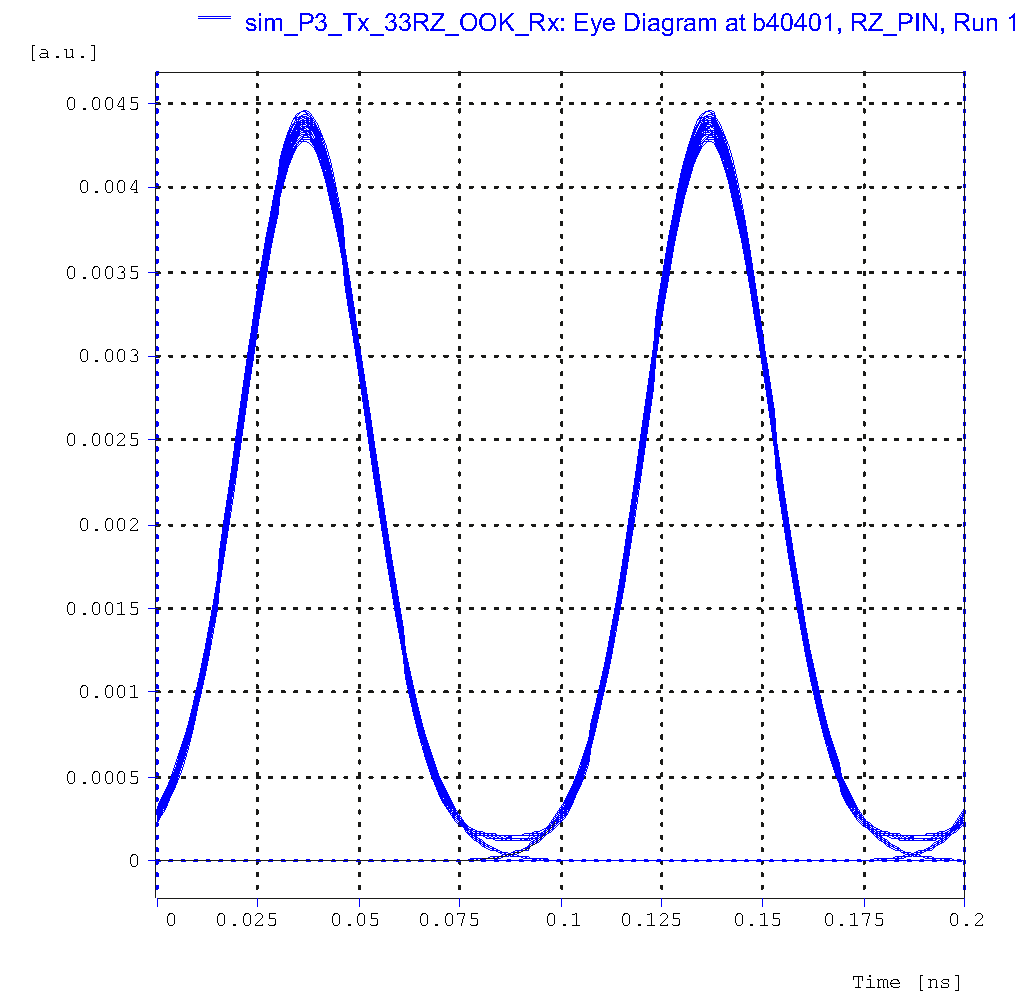
\includegraphics[totalheight=6 cm]{Grafiken/P3ExB_Eye10.pdf}\label{fig:P3ExB_Eye10}~}
	\subfloat[20 km]{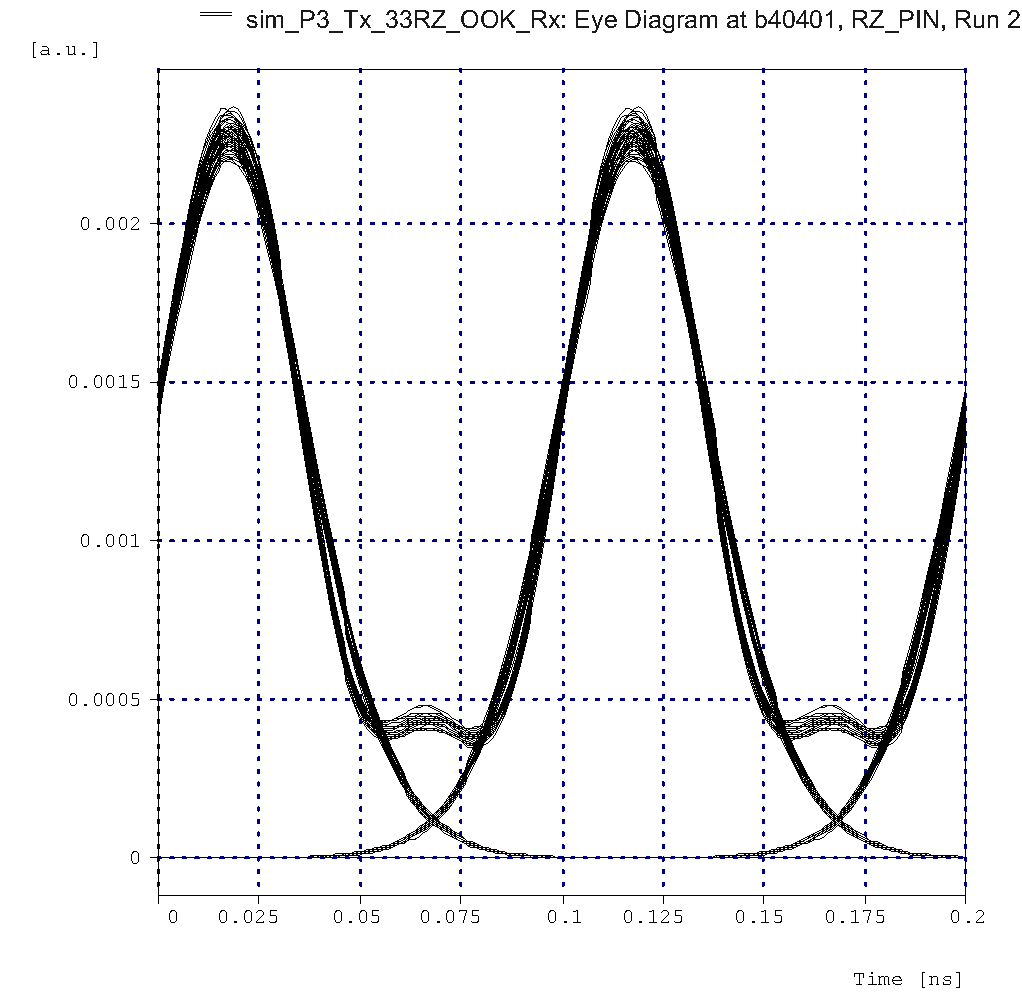
\includegraphics[totalheight=6 cm]{Grafiken/P3ExB_Eye20.pdf} \label{fig:P3ExB_Eye20}}%
%\end{adjustwidth}
\caption{Eye Diagrams after \textbf{a)} 10~km and \textbf{b)} 20~km fibre lenght.}
\label{fig:P3ExB_Eye}%
\end{figure}


\begin{figure}%
\centering
%\begin{adjustwidth}{0cm}{0cm}
	\subfloat[\textit{Q}-factor vs. fibre lenght]{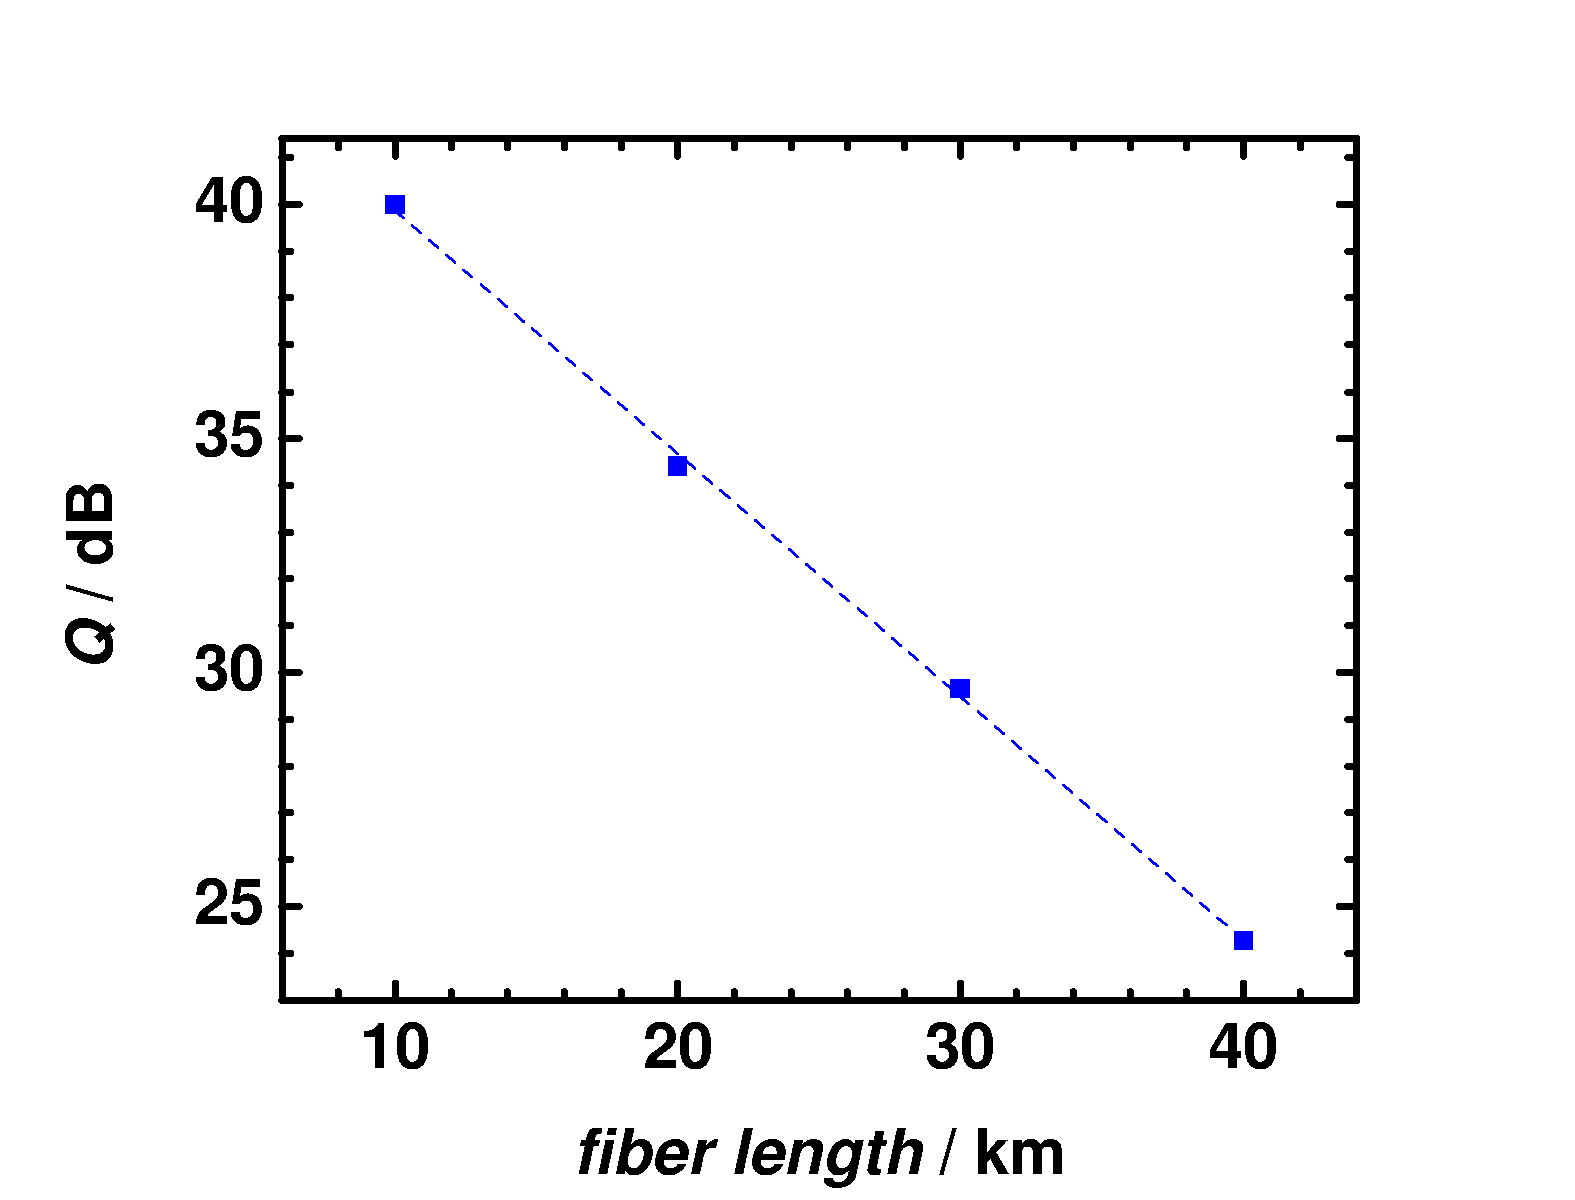
\includegraphics[totalheight=6 cm]{Grafiken/P3ExB_Q.pdf}\label{fig:P3ExB_Q}~}
	\subfloat[\textit{Q}-factor vs. FWHM of the optical source]{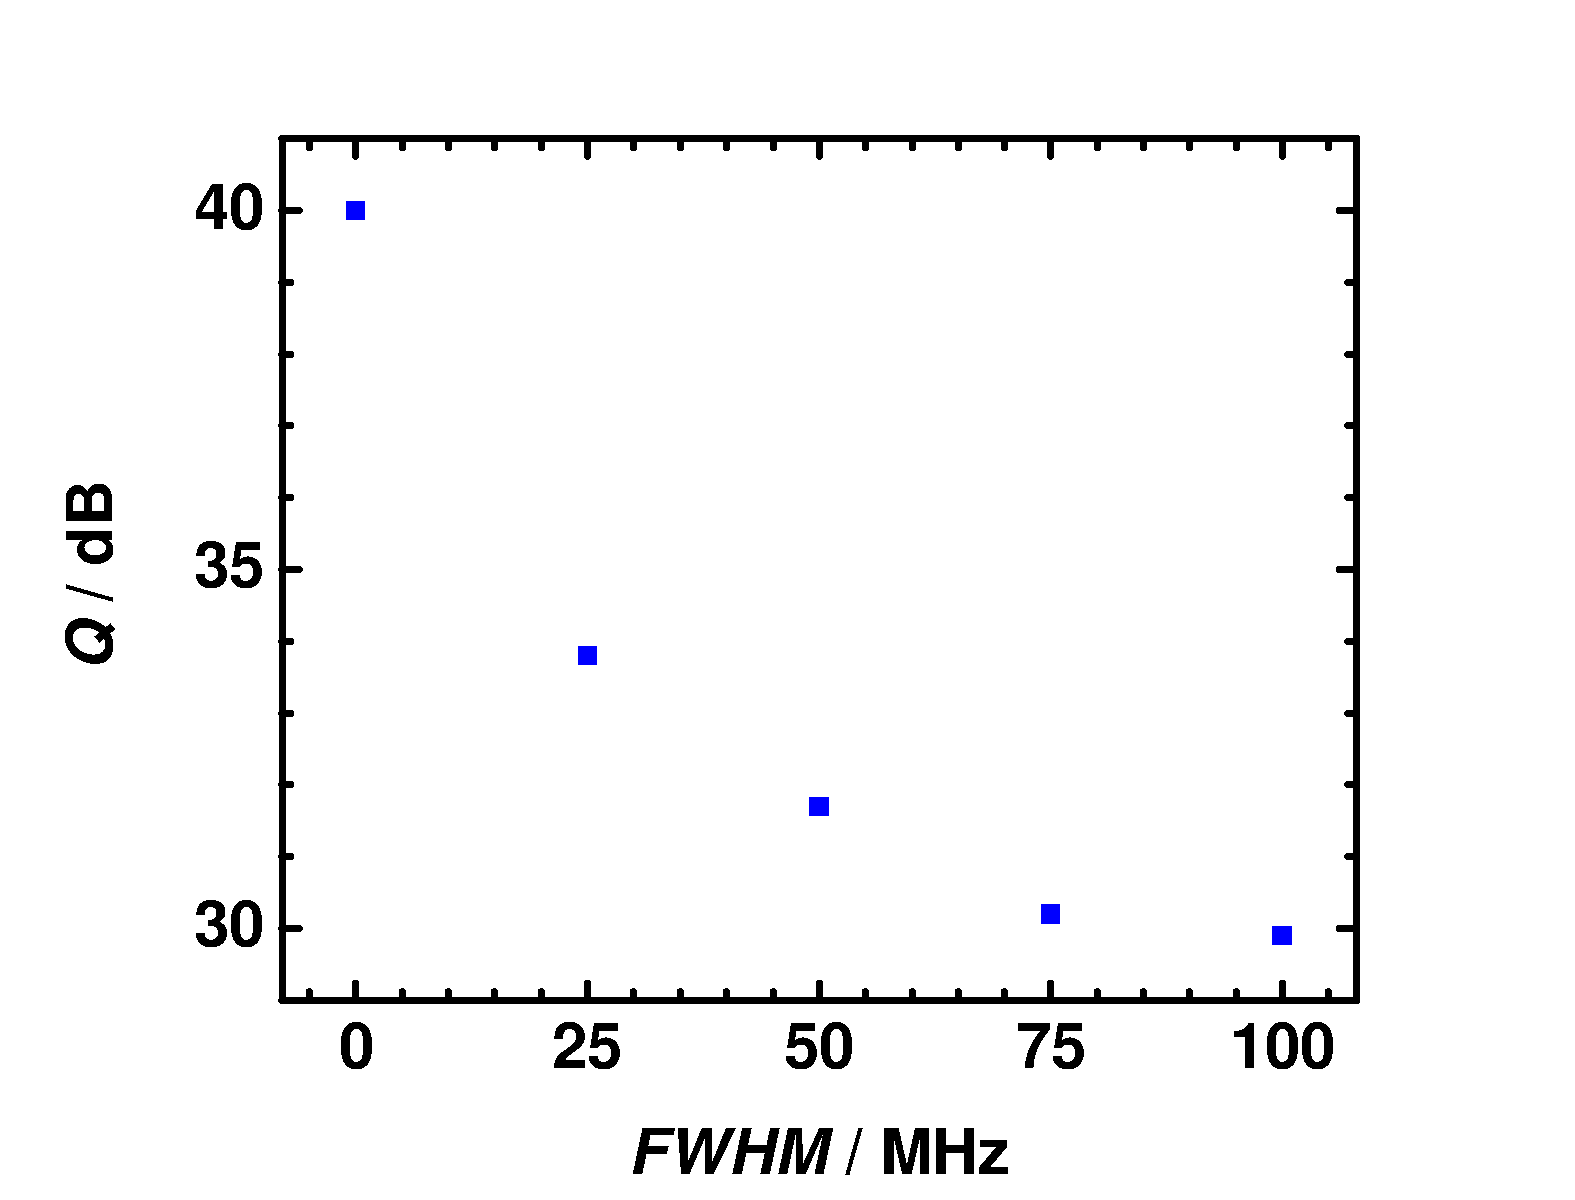
\includegraphics[totalheight=6 cm]{Grafiken/P3ExC_Q.pdf} \label{fig:P3ExC_Q}}%
%\end{adjustwidth}
\caption{\textit{Q}-factors of the optical signal.}
\label{fig:P3_Q}%
\end{figure}

Table \ref{tab:P3ExB_loss} shows the calculated and the measured losses of the fibre with different fibre lengths. For the calculation a attenuation of $\alpha_0=0.19$~dB/km was used. The measured losses are a little bit smaller then the calculated values. This could be caused by \todo{Warum sind die unterschiedlich?}

Because of the fiber there is also a broadening of the transmitted pulse. To examine the influence of the spectral FWHM of the optical source on the transmission characteristic different spectral widths of the laser source were used. The \textit{Q}-factor was measured behind the PIN-diode. In Figure \ref{fig:P3ExC_Q} the logarithmic \textit{Q}-factor is shown at different FWHMs. The \textit{Q}-factor decreases fast with increasing FWHM of the optical source. At a FWHM of $\sim$75~MHz $Q$ reaches 30~dB and stops decreasing so fast and is nearly constant.

To measure the impulse's emporal half-maximum full-width differenz $\Delta t_{\mathrm{H}}$ a prepared bit sequence was loaded ("`costum\_1.dat"') and a parameter scan was performet for the lenght of 10, 20, 30 and 40~km.
The values of $\Delta t_{\mathrm{H}}$ were calculated with
\begin{equation}
\Delta t_{\mathrm{H}} = L\cdot((C\cdot\Delta\lambda)+(D\cdot\Delta\lambda^2))
\label{eq:delta_t}
\end{equation}
where $L$ is the length of the fibre, $C$ is the chromatic dispersion, $D$ is the Derivative of the chromatic dispersion and $\Delta\lambda$ is the spectral range of the signal. The used values were $C=16~\frac{\mathrm{ps}}{\mathrm{nm}\cdot \mathrm{km}}$, $D=0.086~\frac{\mathrm{ps}}{\mathrm{nm}^2\cdot \mathrm{km}}$ and $\Delta\lambda=0.124$~nm are given in the materials for the preparation\footnotemark[3].

\begin{table}%
\centering
\caption{Losses and temporal FWHM differences}
\begin{tabular}{ccccc}

\toprule
Fibre length & Loss in dB&&$\Delta t_{\mathrm{H}}$ in ps&\\
in km&Calculated&Measured&Calculated&Measured\\
\midrule
10&	1.9&1.72&19,85	&2	\\
20&	3.8&3.58&39,7	&	10\\
30&	5.7&5.31&59,56	&	28\\
40&	7.6&7.19&79,41	&	47\\
\bottomrule 
\end{tabular}
\label{tab:P3ExB_loss}
\end{table}


Table \ref{tab:P3ExB_loss} shows the calculated and the measured broadening of the pulses. With a larger fibre-length the temporal FWHM difference gets larger. But there is a large difference between the calculated and the measured values. \todo{Warum sind die Werte so viel anders????}